\secytion{Studio della risoluzione temporale al variare dell'energia}

Una volta ultimata la calibrazione, si è voluto andare a stimare la risoluzione temporale dell'apparato al variare dell'energia depositata sui
rivelatori. Per farlo, si sono analizzati i dati con riferimento all'energia depositata all'interno dei rivelatori: quando la media dell'energia
depositata nei due rivelatori era sopra una certa soglia (o al di fuori della finestra prescelta) si è rimosso tale dato dal campione: ripetendo più
volte questo procedimento al variare della soglia e al variare della finestra è stato possibile stimare la risoluzione temporale. Tale
risoluzione è stata stimata andando a fare un'interpolazione gaussiana dei dati ottenuti in uscita dal TAC, selezionati come precedentemente descritto.
Dato che tale calcolo è stato fatto per molti intervalli di energia, non si riportano qui tutti i grafici creati ma si possono trovare nelle appendici,
mentre nella tabella si possono leggere i risultati ottenuti.
%
\begin{tabella}
	\centering
	\begin{figure}[h] \centering\includegraphics[width=0.9\textwidth]{../../graphs/cobalto_risultati.tex}\caption{cobalto risultati}\label{gr:cobalto_risultati} \end{figure}

	\caption{La risoluzione temporale in funzione dell'energia}
	\label{tab:01tab1}
\end{tabella}
%
Nel grafico sottostante, inoltre, si possono vedere i risultatin dell'analisi, cioè la risoluzione al variare dell'energia rappresentati su un grafico. Si
vede con evidenza che la risoluzione tende a decrescere all'aumentare dell'energia.
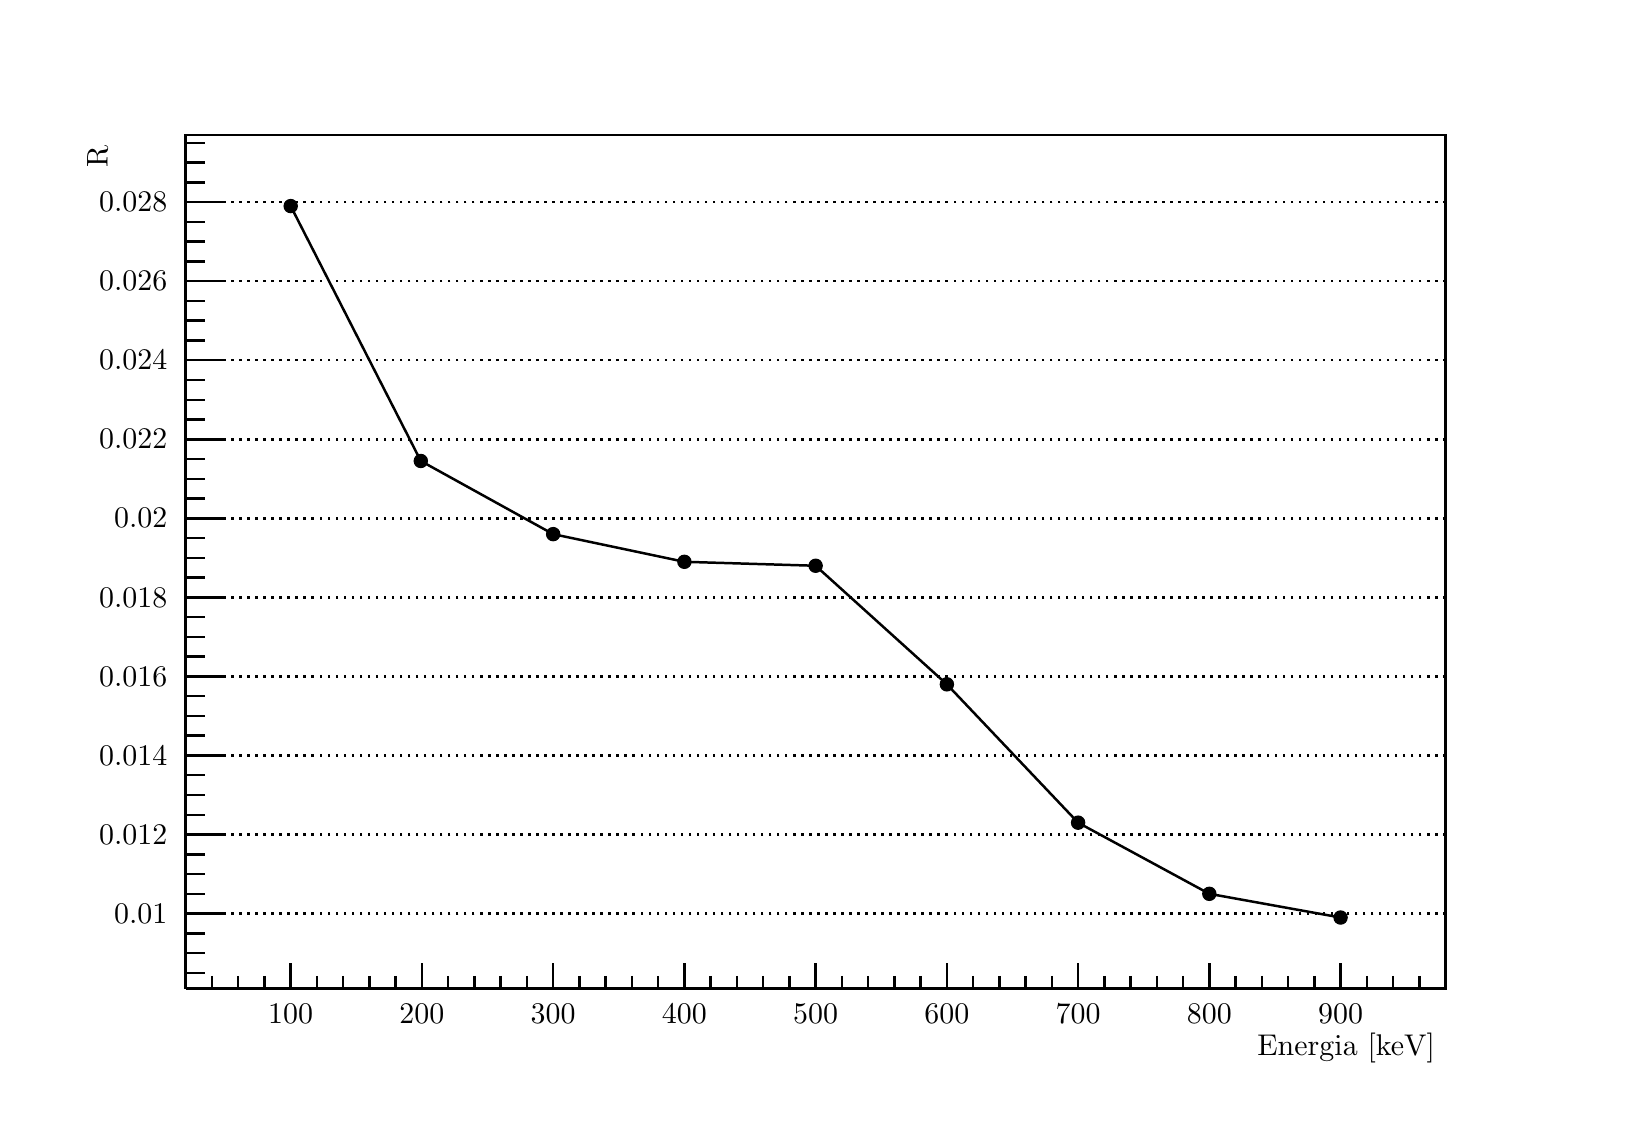
\begin{tikzpicture}
\pgfdeclareplotmark{cross} {
\pgfpathmoveto{\pgfpoint{-0.3\pgfplotmarksize}{\pgfplotmarksize}}
\pgfpathlineto{\pgfpoint{+0.3\pgfplotmarksize}{\pgfplotmarksize}}
\pgfpathlineto{\pgfpoint{+0.3\pgfplotmarksize}{0.3\pgfplotmarksize}}
\pgfpathlineto{\pgfpoint{+1\pgfplotmarksize}{0.3\pgfplotmarksize}}
\pgfpathlineto{\pgfpoint{+1\pgfplotmarksize}{-0.3\pgfplotmarksize}}
\pgfpathlineto{\pgfpoint{+0.3\pgfplotmarksize}{-0.3\pgfplotmarksize}}
\pgfpathlineto{\pgfpoint{+0.3\pgfplotmarksize}{-1.\pgfplotmarksize}}
\pgfpathlineto{\pgfpoint{-0.3\pgfplotmarksize}{-1.\pgfplotmarksize}}
\pgfpathlineto{\pgfpoint{-0.3\pgfplotmarksize}{-0.3\pgfplotmarksize}}
\pgfpathlineto{\pgfpoint{-1.\pgfplotmarksize}{-0.3\pgfplotmarksize}}
\pgfpathlineto{\pgfpoint{-1.\pgfplotmarksize}{0.3\pgfplotmarksize}}
\pgfpathlineto{\pgfpoint{-0.3\pgfplotmarksize}{0.3\pgfplotmarksize}}
\pgfpathclose
\pgfusepathqstroke
}
\pgfdeclareplotmark{cross*} {
\pgfpathmoveto{\pgfpoint{-0.3\pgfplotmarksize}{\pgfplotmarksize}}
\pgfpathlineto{\pgfpoint{+0.3\pgfplotmarksize}{\pgfplotmarksize}}
\pgfpathlineto{\pgfpoint{+0.3\pgfplotmarksize}{0.3\pgfplotmarksize}}
\pgfpathlineto{\pgfpoint{+1\pgfplotmarksize}{0.3\pgfplotmarksize}}
\pgfpathlineto{\pgfpoint{+1\pgfplotmarksize}{-0.3\pgfplotmarksize}}
\pgfpathlineto{\pgfpoint{+0.3\pgfplotmarksize}{-0.3\pgfplotmarksize}}
\pgfpathlineto{\pgfpoint{+0.3\pgfplotmarksize}{-1.\pgfplotmarksize}}
\pgfpathlineto{\pgfpoint{-0.3\pgfplotmarksize}{-1.\pgfplotmarksize}}
\pgfpathlineto{\pgfpoint{-0.3\pgfplotmarksize}{-0.3\pgfplotmarksize}}
\pgfpathlineto{\pgfpoint{-1.\pgfplotmarksize}{-0.3\pgfplotmarksize}}
\pgfpathlineto{\pgfpoint{-1.\pgfplotmarksize}{0.3\pgfplotmarksize}}
\pgfpathlineto{\pgfpoint{-0.3\pgfplotmarksize}{0.3\pgfplotmarksize}}
\pgfpathclose
\pgfusepathqfillstroke
}
\pgfdeclareplotmark{newstar} {
\pgfpathmoveto{\pgfqpoint{0pt}{\pgfplotmarksize}}
\pgfpathlineto{\pgfqpointpolar{44}{0.5\pgfplotmarksize}}
\pgfpathlineto{\pgfqpointpolar{18}{\pgfplotmarksize}}
\pgfpathlineto{\pgfqpointpolar{-20}{0.5\pgfplotmarksize}}
\pgfpathlineto{\pgfqpointpolar{-54}{\pgfplotmarksize}}
\pgfpathlineto{\pgfqpointpolar{-90}{0.5\pgfplotmarksize}}
\pgfpathlineto{\pgfqpointpolar{234}{\pgfplotmarksize}}
\pgfpathlineto{\pgfqpointpolar{198}{0.5\pgfplotmarksize}}
\pgfpathlineto{\pgfqpointpolar{162}{\pgfplotmarksize}}
\pgfpathlineto{\pgfqpointpolar{134}{0.5\pgfplotmarksize}}
\pgfpathclose
\pgfusepathqstroke
}
\pgfdeclareplotmark{newstar*} {
\pgfpathmoveto{\pgfqpoint{0pt}{\pgfplotmarksize}}
\pgfpathlineto{\pgfqpointpolar{44}{0.5\pgfplotmarksize}}
\pgfpathlineto{\pgfqpointpolar{18}{\pgfplotmarksize}}
\pgfpathlineto{\pgfqpointpolar{-20}{0.5\pgfplotmarksize}}
\pgfpathlineto{\pgfqpointpolar{-54}{\pgfplotmarksize}}
\pgfpathlineto{\pgfqpointpolar{-90}{0.5\pgfplotmarksize}}
\pgfpathlineto{\pgfqpointpolar{234}{\pgfplotmarksize}}
\pgfpathlineto{\pgfqpointpolar{198}{0.5\pgfplotmarksize}}
\pgfpathlineto{\pgfqpointpolar{162}{\pgfplotmarksize}}
\pgfpathlineto{\pgfqpointpolar{134}{0.5\pgfplotmarksize}}
\pgfpathclose
\pgfusepathqfillstroke
}
\definecolor{c}{rgb}{1,1,1};
\draw [color=c, fill=c] (0,0) rectangle (20,13.553);
\draw [color=c, fill=c] (2,1.3553) rectangle (18,12.1977);
\definecolor{c}{rgb}{0,0,0};
\draw [c,line width=0.9] (2,1.3553) -- (2,12.1977) -- (18,12.1977) -- (18,1.3553) -- (2,1.3553);
\definecolor{c}{rgb}{1,1,1};
\draw [color=c, fill=c] (2,1.3553) rectangle (18,12.1977);
\definecolor{c}{rgb}{0,0,0};
\draw [c,line width=0.9] (2,1.3553) -- (2,12.1977) -- (18,12.1977) -- (18,1.3553) -- (2,1.3553);
\draw [c,line width=0.9] (2,1.3553) -- (18,1.3553);
\draw [c,line width=0.9] (2,1.3553) -- (2,12.1977);
\draw [c,dotted,line width=0.9] (18,2.30903) -- (2,2.30903);
\draw [c,dotted,line width=0.9] (18,3.31296) -- (2,3.31296);
\draw [c,dotted,line width=0.9] (18,4.31688) -- (2,4.31688);
\draw [c,dotted,line width=0.9] (18,5.32081) -- (2,5.32081);
\draw [c,dotted,line width=0.9] (18,6.32474) -- (2,6.32474);
\draw [c,dotted,line width=0.9] (18,7.32866) -- (2,7.32866);
\draw [c,dotted,line width=0.9] (18,8.33259) -- (2,8.33259);
\draw [c,dotted,line width=0.9] (18,9.33652) -- (2,9.33652);
\draw [c,dotted,line width=0.9] (18,10.3404) -- (2,10.3404);
\draw [c,dotted,line width=0.9] (18,11.3444) -- (2,11.3444);
\draw [c,dotted,line width=0.9] (18,2.30903) -- (2,2.30903);
\draw [c,dotted,line width=0.9] (18,11.3444) -- (2,11.3444);
\draw [c,line width=0.9] (2,1.3553) -- (18,1.3553);
\draw [anchor= east] (18,0.596333) node[scale=1.08185, color=c, rotate=0]{Energia [keV]};
\draw [c,line width=0.9] (3.33333,1.68057) -- (3.33333,1.3553);
\draw [c,line width=0.9] (3.66667,1.51794) -- (3.66667,1.3553);
\draw [c,line width=0.9] (4,1.51794) -- (4,1.3553);
\draw [c,line width=0.9] (4.33333,1.51794) -- (4.33333,1.3553);
\draw [c,line width=0.9] (4.66667,1.51794) -- (4.66667,1.3553);
\draw [c,line width=0.9] (5,1.68057) -- (5,1.3553);
\draw [c,line width=0.9] (5.33333,1.51794) -- (5.33333,1.3553);
\draw [c,line width=0.9] (5.66667,1.51794) -- (5.66667,1.3553);
\draw [c,line width=0.9] (6,1.51794) -- (6,1.3553);
\draw [c,line width=0.9] (6.33333,1.51794) -- (6.33333,1.3553);
\draw [c,line width=0.9] (6.66667,1.68057) -- (6.66667,1.3553);
\draw [c,line width=0.9] (7,1.51794) -- (7,1.3553);
\draw [c,line width=0.9] (7.33333,1.51794) -- (7.33333,1.3553);
\draw [c,line width=0.9] (7.66667,1.51794) -- (7.66667,1.3553);
\draw [c,line width=0.9] (8,1.51794) -- (8,1.3553);
\draw [c,line width=0.9] (8.33333,1.68057) -- (8.33333,1.3553);
\draw [c,line width=0.9] (8.66667,1.51794) -- (8.66667,1.3553);
\draw [c,line width=0.9] (9,1.51794) -- (9,1.3553);
\draw [c,line width=0.9] (9.33333,1.51794) -- (9.33333,1.3553);
\draw [c,line width=0.9] (9.66667,1.51794) -- (9.66667,1.3553);
\draw [c,line width=0.9] (10,1.68057) -- (10,1.3553);
\draw [c,line width=0.9] (10.3333,1.51794) -- (10.3333,1.3553);
\draw [c,line width=0.9] (10.6667,1.51794) -- (10.6667,1.3553);
\draw [c,line width=0.9] (11,1.51794) -- (11,1.3553);
\draw [c,line width=0.9] (11.3333,1.51794) -- (11.3333,1.3553);
\draw [c,line width=0.9] (11.6667,1.68057) -- (11.6667,1.3553);
\draw [c,line width=0.9] (12,1.51794) -- (12,1.3553);
\draw [c,line width=0.9] (12.3333,1.51794) -- (12.3333,1.3553);
\draw [c,line width=0.9] (12.6667,1.51794) -- (12.6667,1.3553);
\draw [c,line width=0.9] (13,1.51794) -- (13,1.3553);
\draw [c,line width=0.9] (13.3333,1.68057) -- (13.3333,1.3553);
\draw [c,line width=0.9] (13.6667,1.51794) -- (13.6667,1.3553);
\draw [c,line width=0.9] (14,1.51794) -- (14,1.3553);
\draw [c,line width=0.9] (14.3333,1.51794) -- (14.3333,1.3553);
\draw [c,line width=0.9] (14.6667,1.51794) -- (14.6667,1.3553);
\draw [c,line width=0.9] (15,1.68057) -- (15,1.3553);
\draw [c,line width=0.9] (15.3333,1.51794) -- (15.3333,1.3553);
\draw [c,line width=0.9] (15.6667,1.51794) -- (15.6667,1.3553);
\draw [c,line width=0.9] (16,1.51794) -- (16,1.3553);
\draw [c,line width=0.9] (16.3333,1.51794) -- (16.3333,1.3553);
\draw [c,line width=0.9] (16.6667,1.68057) -- (16.6667,1.3553);
\draw [c,line width=0.9] (3.33333,1.68057) -- (3.33333,1.3553);
\draw [c,line width=0.9] (3,1.51794) -- (3,1.3553);
\draw [c,line width=0.9] (2.66667,1.51794) -- (2.66667,1.3553);
\draw [c,line width=0.9] (2.33333,1.51794) -- (2.33333,1.3553);
\draw [c,line width=0.9] (2,1.51794) -- (2,1.3553);
\draw [c,line width=0.9] (16.6667,1.68057) -- (16.6667,1.3553);
\draw [c,line width=0.9] (17,1.51794) -- (17,1.3553);
\draw [c,line width=0.9] (17.3333,1.51794) -- (17.3333,1.3553);
\draw [c,line width=0.9] (17.6667,1.51794) -- (17.6667,1.3553);
\draw [c,line width=0.9] (18,1.51794) -- (18,1.3553);
\draw [anchor=base] (3.33333,0.908052) node[scale=1.08185, color=c, rotate=0]{100};
\draw [anchor=base] (5,0.908052) node[scale=1.08185, color=c, rotate=0]{200};
\draw [anchor=base] (6.66667,0.908052) node[scale=1.08185, color=c, rotate=0]{300};
\draw [anchor=base] (8.33333,0.908052) node[scale=1.08185, color=c, rotate=0]{400};
\draw [anchor=base] (10,0.908052) node[scale=1.08185, color=c, rotate=0]{500};
\draw [anchor=base] (11.6667,0.908052) node[scale=1.08185, color=c, rotate=0]{600};
\draw [anchor=base] (13.3333,0.908052) node[scale=1.08185, color=c, rotate=0]{700};
\draw [anchor=base] (15,0.908052) node[scale=1.08185, color=c, rotate=0]{800};
\draw [anchor=base] (16.6667,0.908052) node[scale=1.08185, color=c, rotate=0]{900};
\draw [c,line width=0.9] (2,1.3553) -- (2,12.1977);
\draw [anchor= east] (0.88,12.1977) node[scale=1.08185, color=c, rotate=90]{R};
\draw [c,line width=0.9] (2.48,2.30903) -- (2,2.30903);
\draw [c,line width=0.9] (2.24,2.56001) -- (2,2.56001);
\draw [c,line width=0.9] (2.24,2.81099) -- (2,2.81099);
\draw [c,line width=0.9] (2.24,3.06198) -- (2,3.06198);
\draw [c,line width=0.9] (2.48,3.31296) -- (2,3.31296);
\draw [c,line width=0.9] (2.24,3.56394) -- (2,3.56394);
\draw [c,line width=0.9] (2.24,3.81492) -- (2,3.81492);
\draw [c,line width=0.9] (2.24,4.0659) -- (2,4.0659);
\draw [c,line width=0.9] (2.48,4.31688) -- (2,4.31688);
\draw [c,line width=0.9] (2.24,4.56787) -- (2,4.56787);
\draw [c,line width=0.9] (2.24,4.81885) -- (2,4.81885);
\draw [c,line width=0.9] (2.24,5.06983) -- (2,5.06983);
\draw [c,line width=0.9] (2.48,5.32081) -- (2,5.32081);
\draw [c,line width=0.9] (2.24,5.57179) -- (2,5.57179);
\draw [c,line width=0.9] (2.24,5.82277) -- (2,5.82277);
\draw [c,line width=0.9] (2.24,6.07376) -- (2,6.07376);
\draw [c,line width=0.9] (2.48,6.32474) -- (2,6.32474);
\draw [c,line width=0.9] (2.24,6.57572) -- (2,6.57572);
\draw [c,line width=0.9] (2.24,6.8267) -- (2,6.8267);
\draw [c,line width=0.9] (2.24,7.07768) -- (2,7.07768);
\draw [c,line width=0.9] (2.48,7.32866) -- (2,7.32866);
\draw [c,line width=0.9] (2.24,7.57965) -- (2,7.57965);
\draw [c,line width=0.9] (2.24,7.83063) -- (2,7.83063);
\draw [c,line width=0.9] (2.24,8.08161) -- (2,8.08161);
\draw [c,line width=0.9] (2.48,8.33259) -- (2,8.33259);
\draw [c,line width=0.9] (2.24,8.58357) -- (2,8.58357);
\draw [c,line width=0.9] (2.24,8.83455) -- (2,8.83455);
\draw [c,line width=0.9] (2.24,9.08554) -- (2,9.08554);
\draw [c,line width=0.9] (2.48,9.33652) -- (2,9.33652);
\draw [c,line width=0.9] (2.24,9.5875) -- (2,9.5875);
\draw [c,line width=0.9] (2.24,9.83848) -- (2,9.83848);
\draw [c,line width=0.9] (2.24,10.0895) -- (2,10.0895);
\draw [c,line width=0.9] (2.48,10.3404) -- (2,10.3404);
\draw [c,line width=0.9] (2.24,10.5914) -- (2,10.5914);
\draw [c,line width=0.9] (2.24,10.8424) -- (2,10.8424);
\draw [c,line width=0.9] (2.24,11.0934) -- (2,11.0934);
\draw [c,line width=0.9] (2.48,11.3444) -- (2,11.3444);
\draw [c,line width=0.9] (2.48,2.30903) -- (2,2.30903);
\draw [c,line width=0.9] (2.24,2.05805) -- (2,2.05805);
\draw [c,line width=0.9] (2.24,1.80707) -- (2,1.80707);
\draw [c,line width=0.9] (2.24,1.55609) -- (2,1.55609);
\draw [c,line width=0.9] (2.48,11.3444) -- (2,11.3444);
\draw [c,line width=0.9] (2.24,11.5954) -- (2,11.5954);
\draw [c,line width=0.9] (2.24,11.8463) -- (2,11.8463);
\draw [c,line width=0.9] (2.24,12.0973) -- (2,12.0973);
\draw [anchor= east] (1.9,2.30903) node[scale=1.08185, color=c, rotate=0]{0.01};
\draw [anchor= east] (1.9,3.31296) node[scale=1.08185, color=c, rotate=0]{0.012};
\draw [anchor= east] (1.9,4.31688) node[scale=1.08185, color=c, rotate=0]{0.014};
\draw [anchor= east] (1.9,5.32081) node[scale=1.08185, color=c, rotate=0]{0.016};
\draw [anchor= east] (1.9,6.32474) node[scale=1.08185, color=c, rotate=0]{0.018};
\draw [anchor= east] (1.9,7.32866) node[scale=1.08185, color=c, rotate=0]{0.02};
\draw [anchor= east] (1.9,8.33259) node[scale=1.08185, color=c, rotate=0]{0.022};
\draw [anchor= east] (1.9,9.33652) node[scale=1.08185, color=c, rotate=0]{0.024};
\draw [anchor= east] (1.9,10.3404) node[scale=1.08185, color=c, rotate=0]{0.026};
\draw [anchor= east] (1.9,11.3444) node[scale=1.08185, color=c, rotate=0]{0.028};
\draw [c,line width=0.9] (3.33333,11.2942) -- (4.98567,8.05699) -- (6.66667,7.12788) -- (8.33333,6.7765) -- (10,6.72631) -- (11.6667,5.22042) -- (13.3333,3.46355) -- (15,2.56001) -- (16.6667,2.25884);
\foreach \P in {(3.33333,11.2942), (4.98567,8.05699), (6.66667,7.12788), (8.33333,6.7765), (10,6.72631), (11.6667,5.22042), (13.3333,3.46355), (15,2.56001), (16.6667,2.25884)}{\draw[mark options={color=c,fill=c},mark size=2.402402pt,mark=*] plot
 coordinates {\P};}
\end{tikzpicture}
\\
